

\section{Introduction}
\index{Scenario Risk}
The scenario risk calculator is capable of computing losses and loss statistics from a single event for a collection of assets, given a set of \glspl{groundmotionfield}. The use of a set of \glspl{groundmotionfield} is recommended so that the aleatory variability (both inter- and intra-event) in the \gls{groundmotionpredictioneq} is modelled. The input glspl{groundmotionfield} can be calculated with oq-hazardlib or by an external software; in either case they need to be stored in the OpenQuake engine database. With the use of the oq-hazardlib, these glspl{groundmotionfield} can be calculated either with or without the spatial correlation of the ground motion residuals.

For each gls{groundmotionfield}, the intensity measure level at a given site is combined with a \gls{vulnerability function}, from which a loss ratio is randomly sampled, for each \gls{asset} contained in the \gls{exposure model}. The loss ratios that are sampled for \glspl{asset} of a given \gls{taxonomy} classification at different locations can be considered to be either independent, fully correlated, or correlated with a specific correlation coefficient. Using these results, the mean and standard deviation of the loss ratios across all \glspl{groundmotionfield} can be calculated. Loss ratios are converted into losses by multiplying by the structural value of the \gls{asset} given in the exposure model. It is furthermore possible to sum the losses throughout the region and to compute the mean and standard deviation of the total loss. 

\section{Calculation Steps}

To compute the mean loss:

\begin{enumerate}
\item For each \gls{groundmotionfield}, the intensity measure level at the location of the \gls{asset} is used to derive the mean loss ratio and associated coefficient of variation from the \gls{vulnerability function}. Since currently the \glspl{vulnerability function} are being defined in a discrete manner, it is quite probable that the intensity measure level provided by the \gls{groundmotionfield} is not contained in the \gls{vulnerability function}. In these cases, linear interpolation methods are being employed to derive the mean loss ratio at the intensity measure level of interest. 

\item The engine takes the \gls{vulnerability function} assigned to each \gls{asset} and checks if the coefficient of variation is zero. If so, the loss ratios are derived based on the mean loss ratio for each intensity measure level. Otherwise, if the uncertainty is defined, it is randomly sampled following the probabilistic distribution of the respective \gls{vulnerability function}, as described below:

\begin{equation}
\log{LR_n} = \mu + \epsilon\sigma
\end{equation}

Where $\mu$ and $\sigma$ stand for the mean and standard deviation of the logarithm of the loss ratios respectively and $\epsilon$ is a term that has a standard normal distribution with a zero mean and a standard deviation of one.  

The method used to sample epsilon depends on whether the correlation between the vulnerability uncertainty of \glspl{asset} of a given \gls{taxonomy} is to be considered or not:

\begin{itemize}

\item Perfectly correlated: the term $\epsilon$ is randomly sampled once for the first \gls{asset} and this result is used to derive the loss ratio for all the \glspl{asset} of the same \gls{taxonomy}. 

\item Correlated: the term $\epsilon$ is randomly sampled for each \gls{asset} considering the specified correlation coefficient between \glspl{asset}. 

\item Uncorrelated: the term $\epsilon$ is always randomly sampled for each \gls{asset} and therefore the correlation between the vulnerability of the \glspl{asset} is ignored.

\end{itemize}

\item The mean loss ratio for each \gls{asset} across all possible simulations of the scenario event can be calculated through the formula:

\begin{equation}
LR=\frac{\sum^m_{n=1}LR_n|IML}{m}
\end{equation}

Where $m$ stands for the number of ground motion fields simulated.

\item The mean loss can then be derived by multiplying the mean loss ratio by the value of the \gls{asset} contained in the \gls{exposure model} file.

\end{enumerate}

To compute the standard deviation of the loss:

\begin{enumerate}

\item In order to compute the uncertainty, the engine takes the set of loss ratios for each \gls{asset}, and computes the associated standard deviation using the classical formula:

\begin{equation}
SD[LR]=\sqrt{  \frac{1}{m}\sum_{n=1}^m{(LR_n-E[LR])^2} }
\end{equation}

Where $E[LR]$ stands for the mean loss ratio computed previously.

\item The standard deviation of the absolute loss can finally be computed by multiplying the standard deviation of the loss ratio by the value of the respective \gls{asset}.

\end{enumerate}

\section{Calculator Output}
The output of the Scenario Risk Calculator currently comprises loss statistics (mean total loss and standard deviation of total loss) and loss maps. Loss maps are comprised by a set of loss nodes, which are associated with a pair of coordinates. For each node, one or more loss values might exist, due to the fact that several different \glspl{asset} can be located at the same location.  Figure \ref{fig:detlosses} presents an example of a loss map containing the expected economic losses for residental buildings located in Nepal, considering a rupture of magnitude 7.0Mw in the central part of the country.

\begin{figure}[ht]
\centering
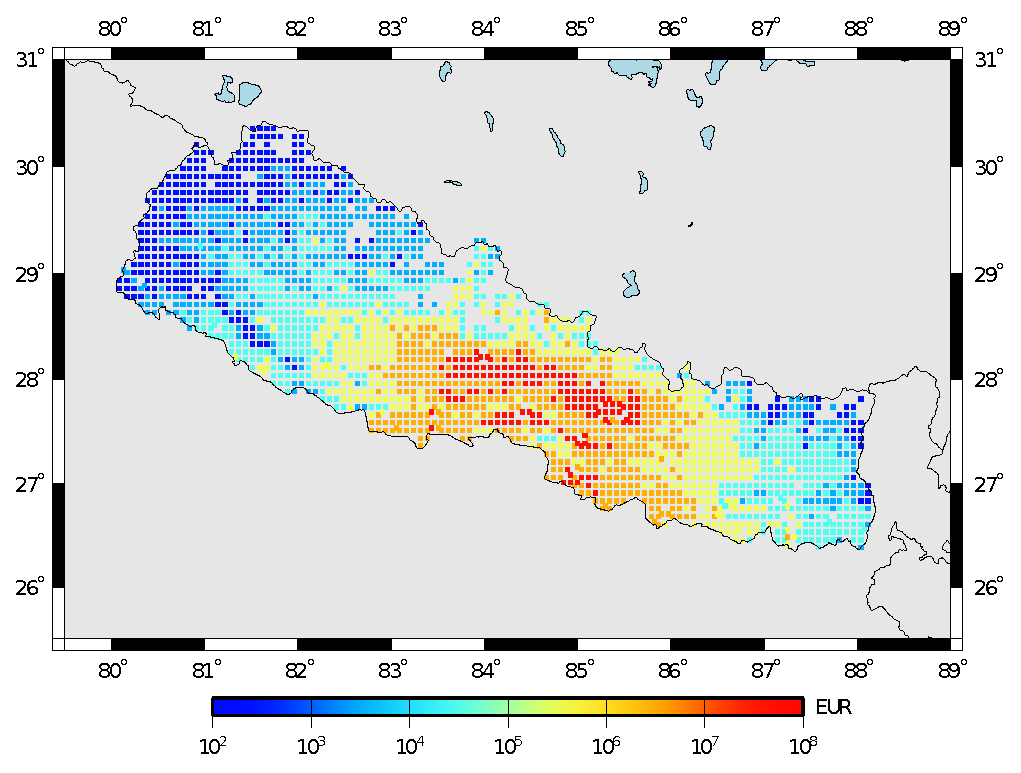
\includegraphics[width=12cm,height=7cm]{./figures/risk/LossmapDet.eps}
\caption{Loss map with the distribution of mean economic losses for residential buildings in Nepal.}
\label{fig:detlosses}
\end{figure} 